\documentclass[11pt]{article}
\usepackage[margin=0.72in]{geometry}
\usepackage{graphicx}
\usepackage{xcolor}
\usepackage{hyperref}
\usepackage{caption}
\usepackage{float}
\usepackage{titlesec}
\usepackage{enumitem}

\definecolor{ink}{HTML}{2B2118}
\definecolor{muted}{HTML}{584A34}
\definecolor{rust}{HTML}{6E2420}
\definecolor{teal}{HTML}{2E6E63}
\definecolor{paper}{HTML}{F6EEDD}
\hypersetup{colorlinks=true, urlcolor=teal, linkcolor=teal}
\captionsetup{font=small, labelfont=bf}
\titleformat{\section}{\large\bfseries\color{ink}}{}{0em}{}
\setlist[itemize]{leftmargin=1.25em, itemsep=0.22em}
\graphicspath{{figures_map/}}
\emergencystretch=3em

\begin{document}

\begin{center}
{\Huge \bfseries The Shorter Way South}\\[0.35em]
{\Large A D3 scrollytelling map of white stork migration from Germany toward Africa}\\[0.75em]
{\color{muted} DSC 106 Final Project Proposal}\\[0.35em]
{\color{muted} Roxanne Wang, Ryan Zhang, Keith Gong}
\end{center}

\section{Project Title}
\textbf{The Shorter Way South}

\section{Dataset URL and Citation}
We will use the Movebank Data Repository dataset \textit{LifeTrack White Stork SW Germany}, DOI:
\href{https://doi.org/10.5441/001/1.ck04mn78}{10.5441/001/1.ck04mn78}, with the related study \textit{``Closer-to-home'' strategy benefits juvenile survival in a long-distance migratory bird}:
\href{https://doi.org/10.1002/ece3.5395}{10.1002/ece3.5395}. The dataset contains GPS bio-logging records for white storks tagged in southwest Germany, including timestamp, longitude, latitude, individual bird identifier, ground speed, and deployment metadata. The full study describes lifetime GPS tracking of 169 white storks; for our interactive prototype, we filtered real GPS fixes from 2013--2019 into 71 complete autumn migration tracks after removing outliers and incomplete/non-migratory records. This dataset is interesting because it turns an ecological change into a spatial story: many storks now shorten migration by wintering in Spain or nearby regions instead of crossing deeper into Africa. The data is also emotionally compelling because each route belongs to an individual animal, so the viewer can move between flock-scale change and one bird's path.

\section{Brief Writeup}
This project will be an interactive map-first scrollytelling experience about white stork migration. Position will always encode real geography: a faint parchment basemap of Europe and Africa anchors every bird path to latitude and longitude. As the reader scrolls, the map will fly from southwest Germany to the western Mediterranean, then reveal the split between birds that cross to Africa and birds that stop closer to home in Spain. A time scrubber will animate the migration season from July to March, while hover interactions reveal an individual bird's ID, date, speed, and full path. The main takeaway is simple and visual: the migration is not disappearing all at once, but it is becoming shorter.

\section{Planned Interactive Experience}
\begin{itemize}
\item \textbf{Map as the stage:} D3 draws Europe and Africa with a geographic projection; all bird positions and paths come from real GPS coordinates.
\item \textbf{Scroll-driven narrative:} steps zoom from the German departure region to the Iberian funnel, the Africa/Spain split, Spain short-stoppers, and Africa crossings.
\item \textbf{Time scrubber:} a labeled July--March range control moves cream bird dots through the season so the flock visibly pours south over time.
\item \textbf{Interaction:} ``Play / Pause,'' ``Show all routes,'' and ``Africa vs Spain'' buttons make the controls readable without hidden labels.
\item \textbf{Hover detail:} hovering a bird highlights only that bird's full route and displays a tooltip with ID, date, migration strategy, and ground speed.
\item \textbf{Color encoding:} seasonal route segments use a gold-to-rust ramp; the key comparison uses rust for Africa crossings and river teal for Spain or short-stopper routes.
\end{itemize}

\section{Static Visualizations from the Prototype}

\begin{figure}[H]
\centering
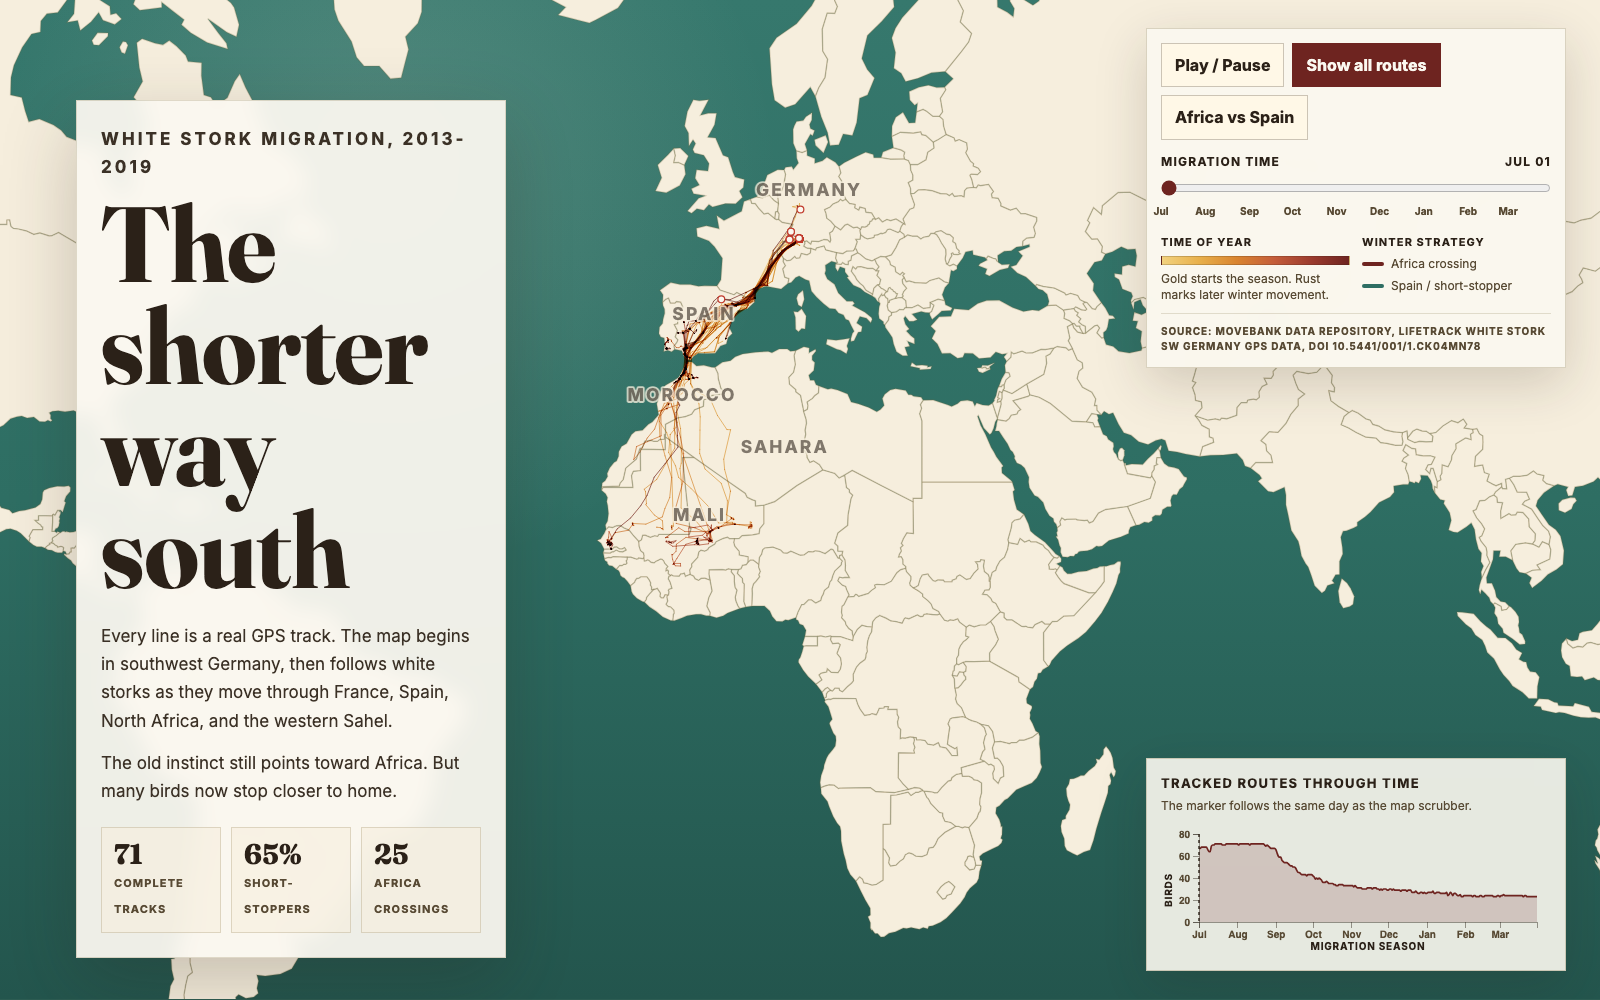
\includegraphics[width=\textwidth]{01_interactive_overview.png}
\caption{\textbf{Interactive overview.} The opening frame places the story card, controls, legends, and real GPS paths on a geographic map of Europe and Africa.}
\end{figure}

\begin{figure}[H]
\centering
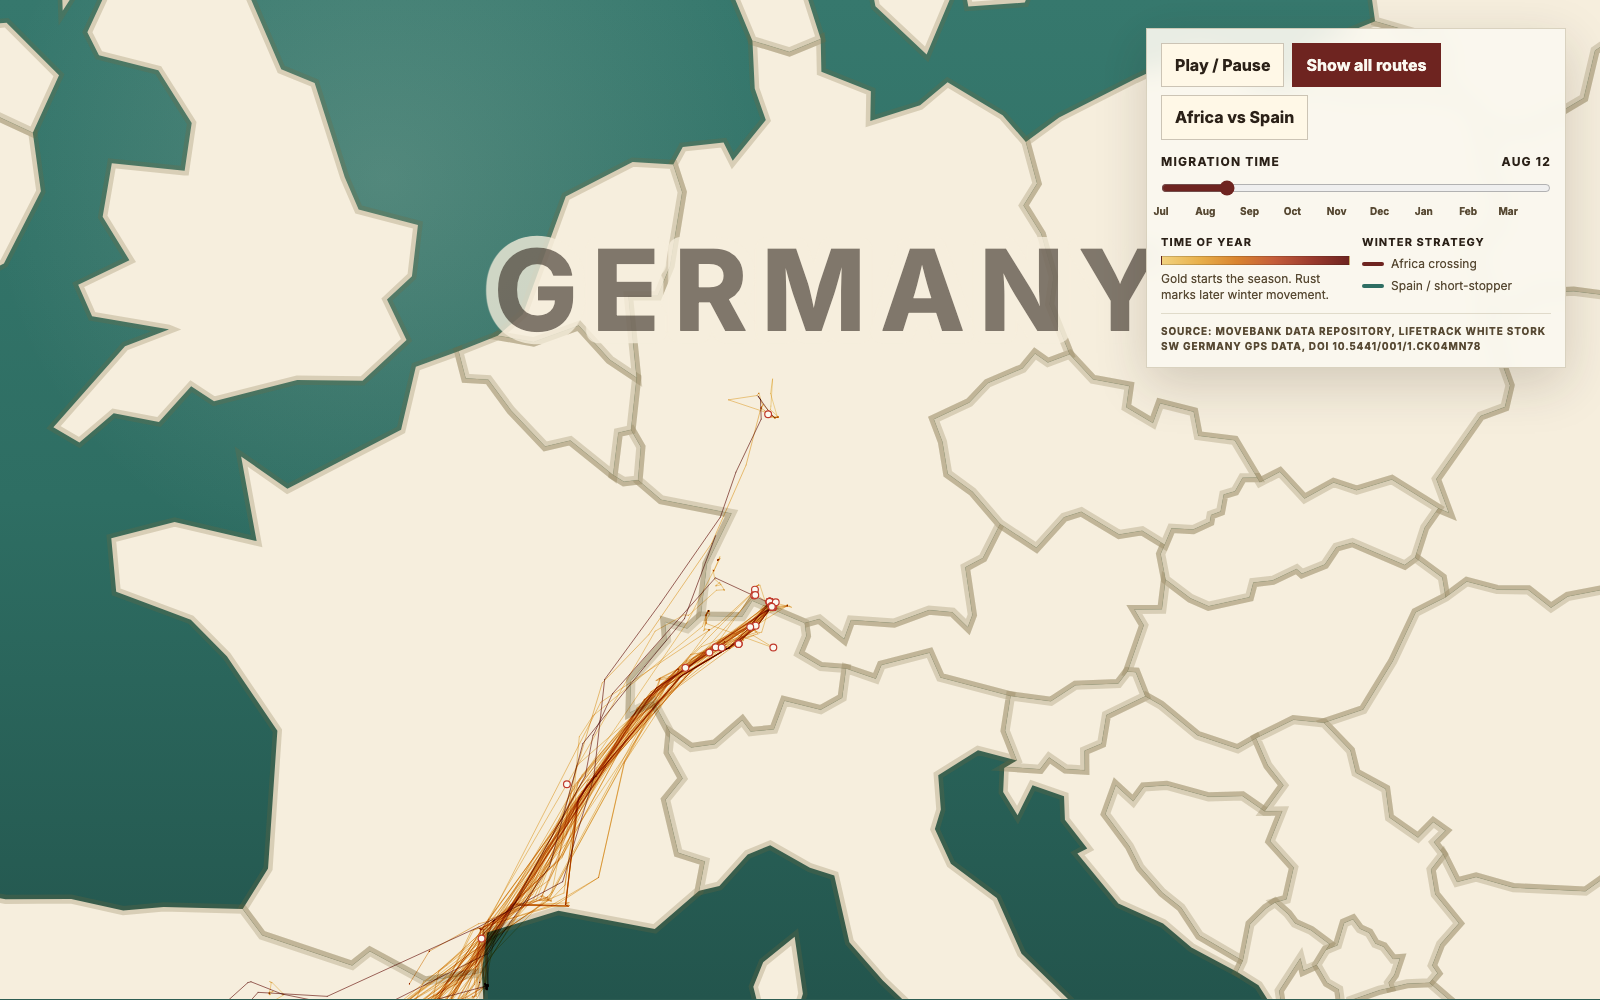
\includegraphics[width=\textwidth]{02_departure_germany.png}
\caption{\textbf{Departure from southwest Germany.} The first scroll step zooms to the real departure geography near southern Germany while the current-position dots remain small and readable.}
\end{figure}

\begin{figure}[H]
\centering
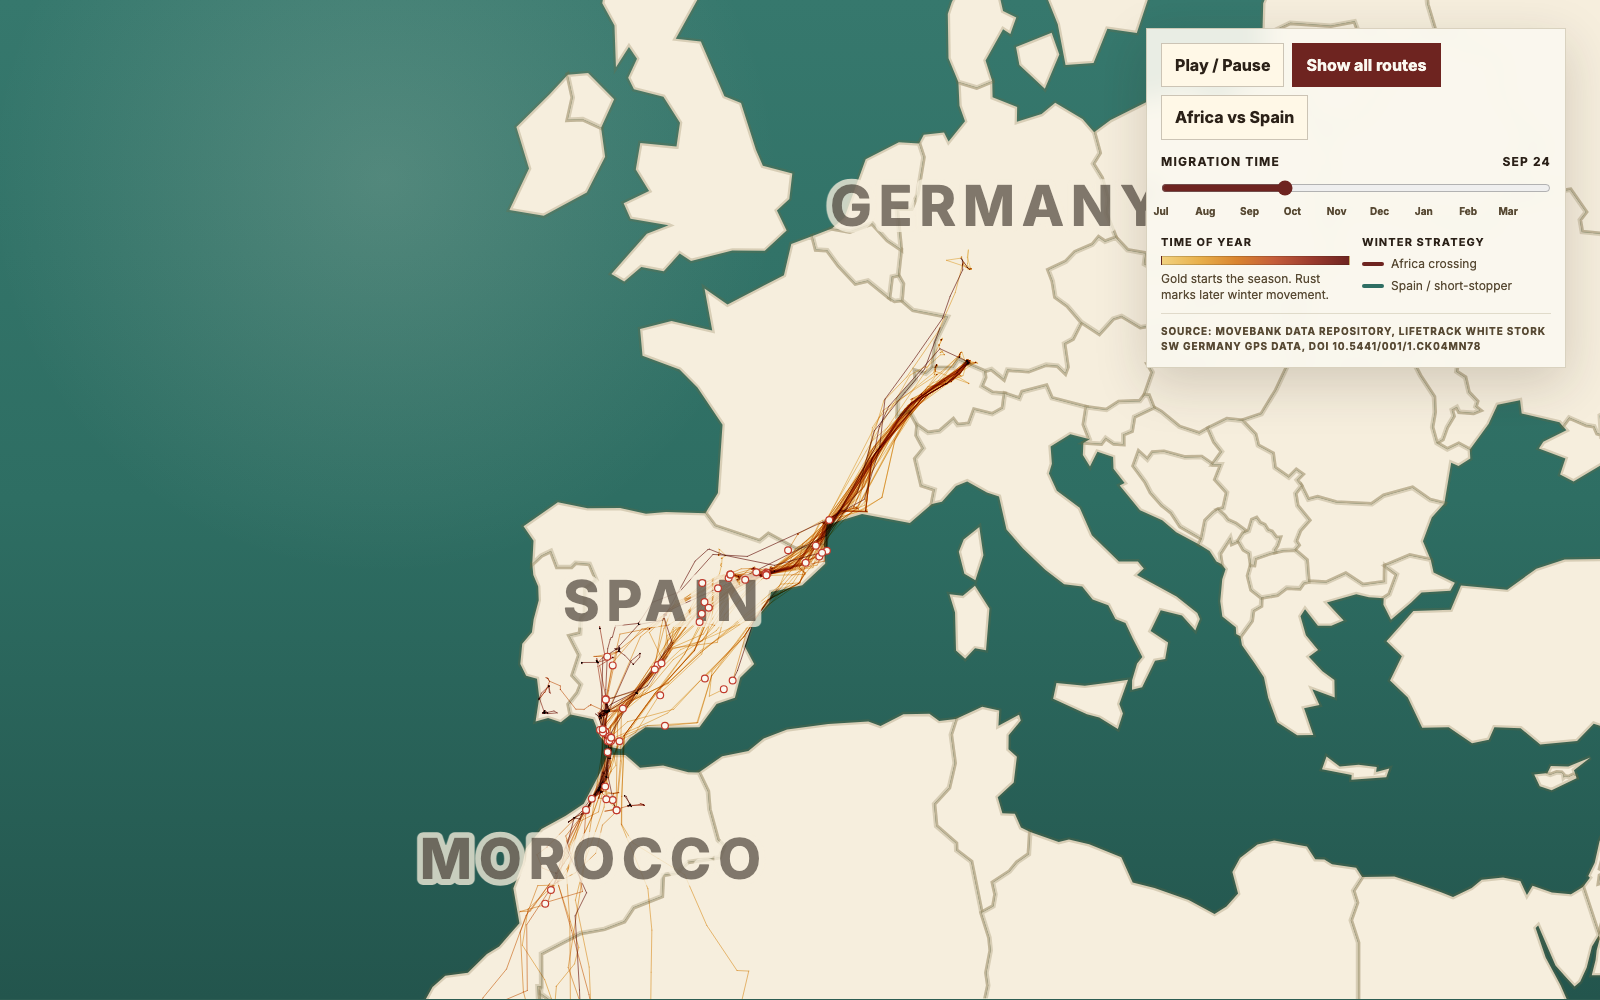
\includegraphics[width=\textwidth]{03_autumn_routes.png}
\caption{\textbf{Autumn route formation.} Seasonal color reveals time: pale gold marks early movement and rust marks later segments as routes funnel toward France, Spain, and North Africa.}
\end{figure}

\begin{figure}[H]
\centering
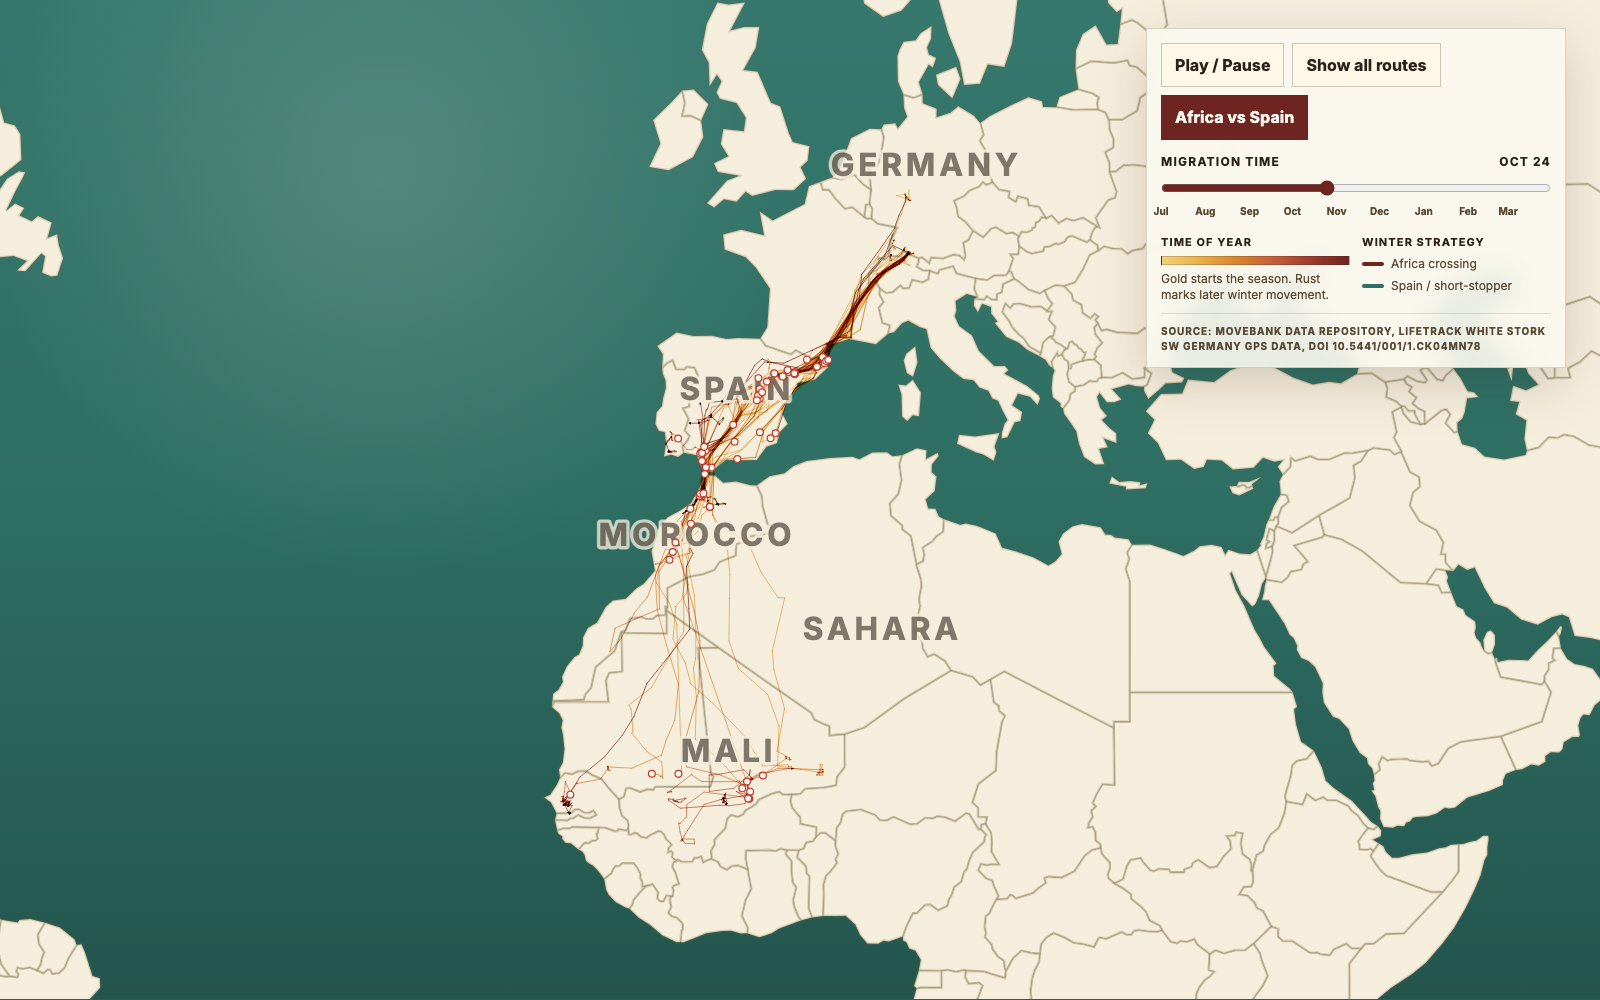
\includegraphics[width=\textwidth]{04_africa_vs_spain_split.png}
\caption{\textbf{Africa vs Spain mode.} The diverging color view separates Africa crossings from Spain or short-stopper routes, making the behavioral split visible on the map.}
\end{figure}

\begin{figure}[H]
\centering
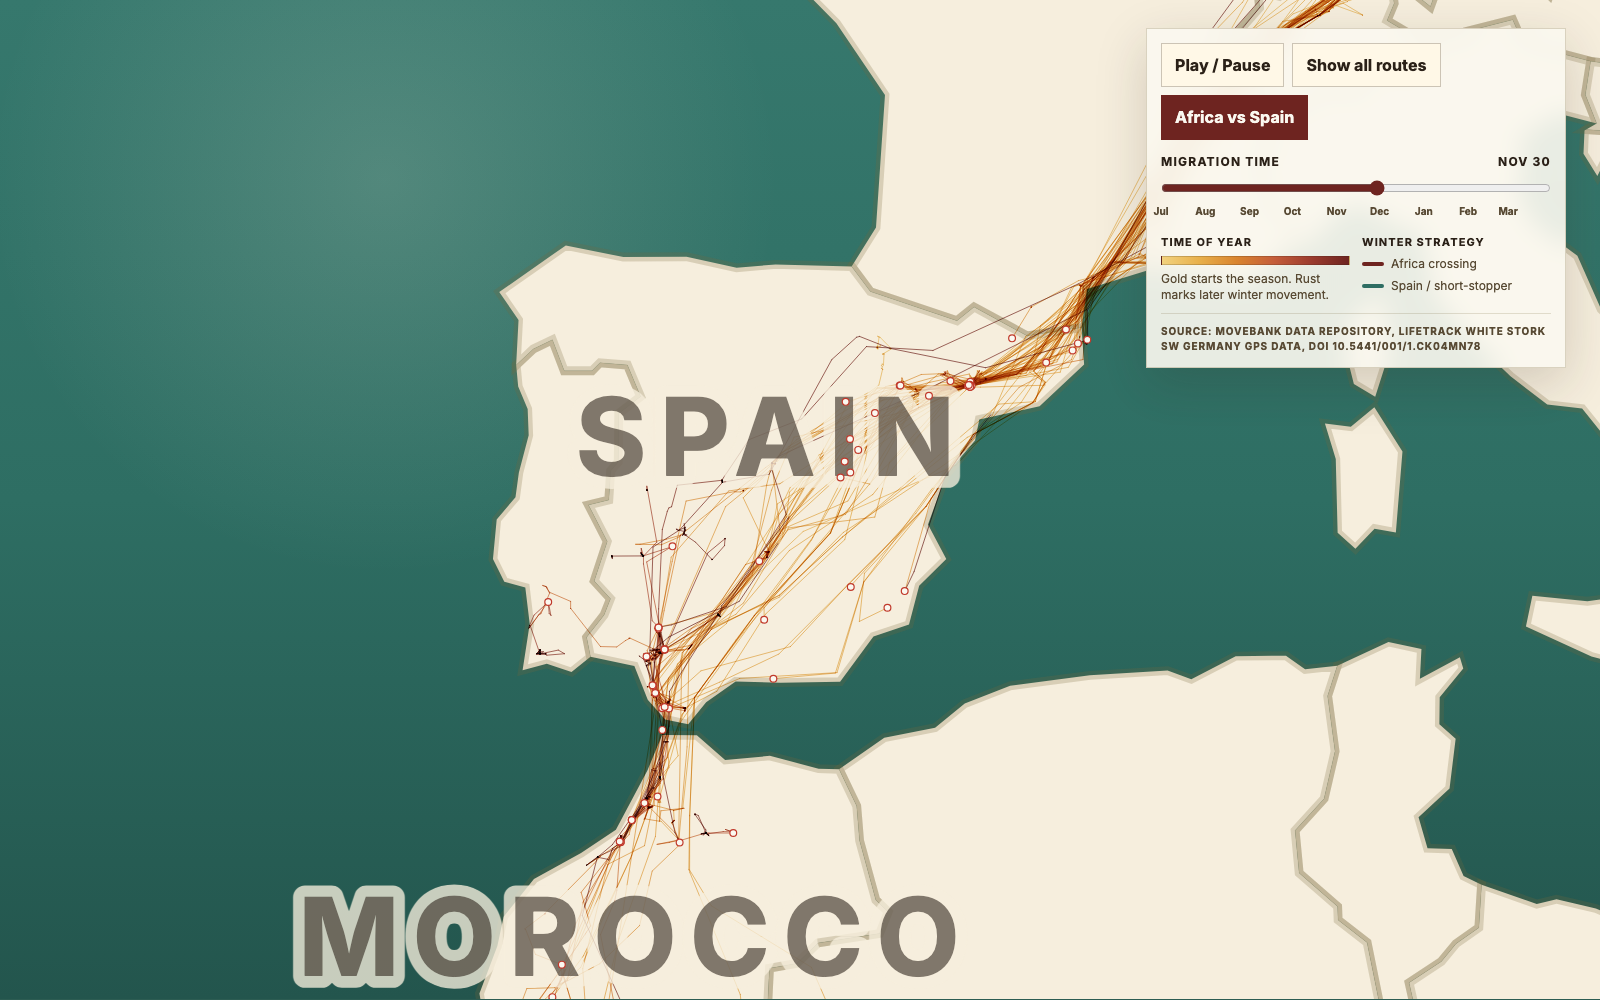
\includegraphics[width=\textwidth]{05_spain_short_stoppers.png}
\caption{\textbf{Closer-to-home wintering.} The Iberian zoom focuses attention on birds that stop around Spain rather than continuing across the Sahara.}
\end{figure}

\begin{figure}[H]
\centering
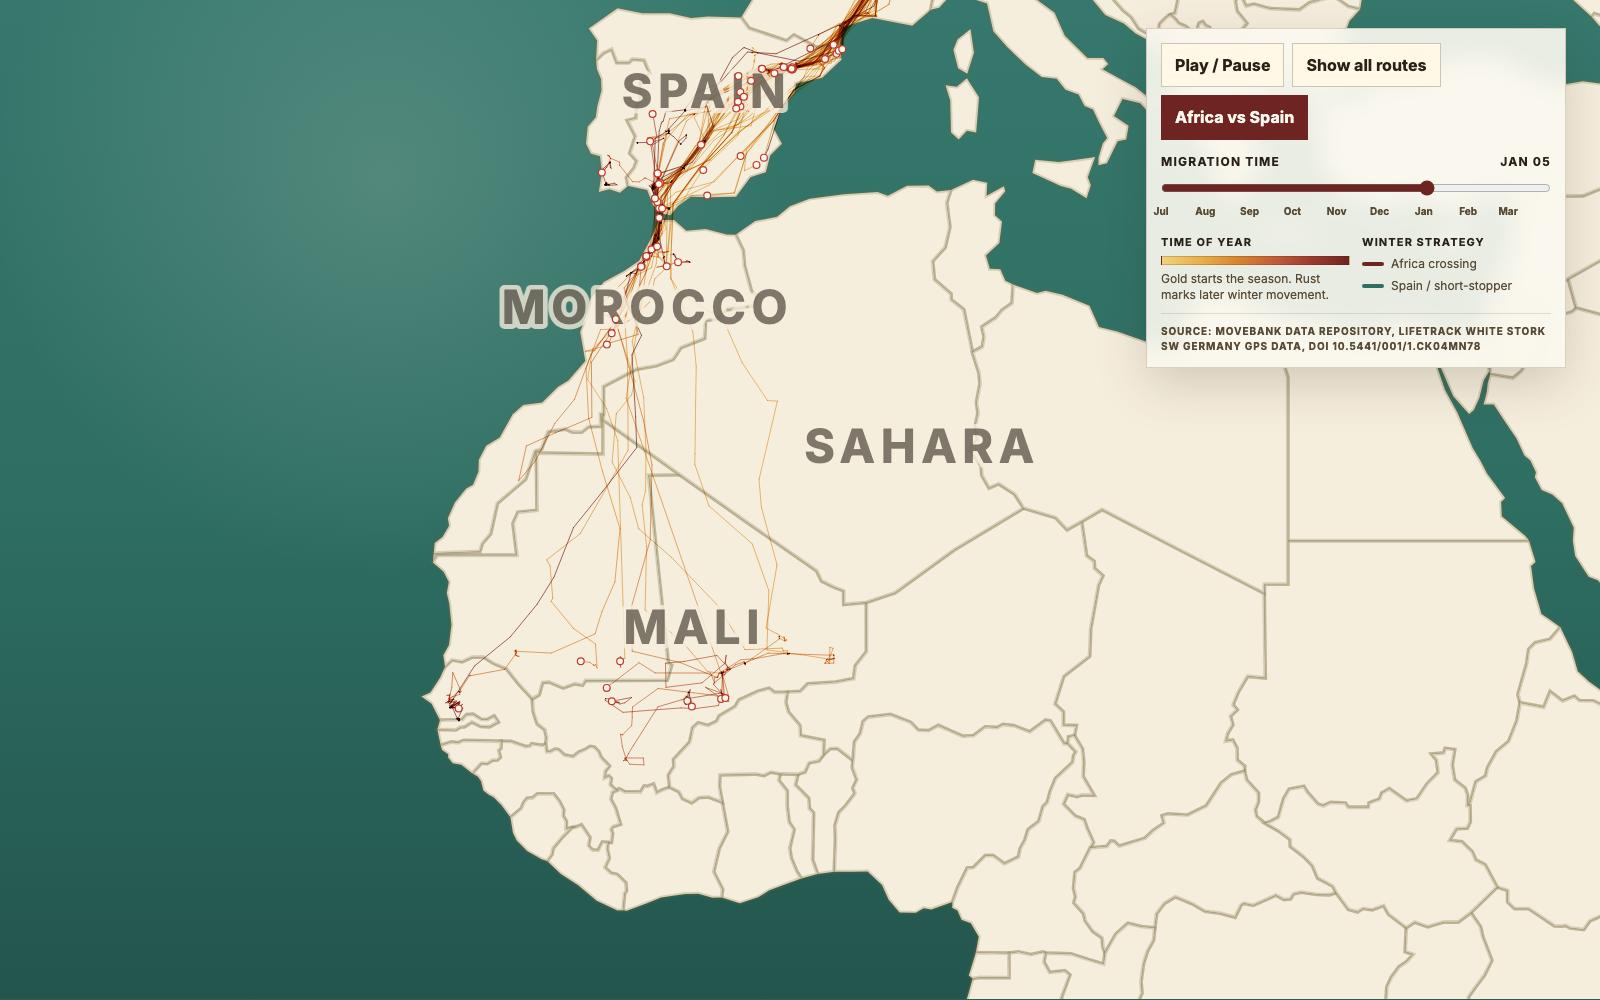
\includegraphics[width=\textwidth]{06_africa_crossings.png}
\caption{\textbf{Africa crossings.} The final map view follows the longer routes across North Africa and into the western Sahel, contrasting the older long-distance path with the shorter strategy.}
\end{figure}

\section{Implementation Plan}
The final explorable will be built with D3.js, TopoJSON world countries, SVG map layers, D3 scales for seasonal and strategy color, IntersectionObserver for scroll steps, and a range input plus timer for playback. The current local prototype is \texttt{stork\_migration\_map.html}; it already loads the processed GPS JSON, renders the basemap, draws route lines, animates current positions, exposes labeled controls, and supports hover highlighting.

\end{document}
